\section {Super-K spectra}
\label{sec:spectra}

\subsection{Definition of Asimov A and B}
\label{sec:asimov_definition}
\Cref{tab:asimov_definition1} shows the definitions used for the Asimov data sets. Asimov A represents a mixture of parameter values at global best fit values and close to the T2K best fit for \PrevRunPeriod, whilst Asimov B modifies these parameters such that CP is conserved and changes the \ssqthtwothree octant.
\begin{table}[H]
\centering
\begin{tabular}{| c | c | c |}
\hline
Parameter(s) &	Asimov A & Asimov B	\\
\hline
$\sin^{2}\theta_{23}$	&	0.528	&  0.450	\\%0.624	\\
$\sin^{2} \theta_{13}$ reactors	&	0.0219	&	0.0219	\\
$\sin^{2} \theta_{12}$	&	0.304	&	0.304	\\
$|\Delta m^{2}_{32}|$ (NH) / $|\Delta m^{2}_{31}|$ (IH)	&	$2.509 \times 10^{-3}~\mbox{eV}^2/\mbox{c}^4$	&	$2.509 \times 10^{-3}~\mbox{eV}^2/\mbox{c}^4$	\\
$\Delta m^{2}_{21}$	&	$7.53 \times 10^{-5}~\mbox{eV}^2/\mbox{c}^4$	&	$7.53 \times 10^{-5}~\mbox{eV}^2/\mbox{c}^4$	\\
$\delta_{CP}$	&	-1.601	&	0	\\
Mass Hierarchy	&	Normal	&	Normal	\\  
\hline
\end{tabular}
\caption{
Values of oscillation parameters used to compute the event rates, systematic effects and sensitivity studies. Each set of oscillation parameters correspond to a different Asimov data set, which is the MC expected distribution in a certain oscillation hypothesis.
In the Asimov data set A the nominal values of $\sin^2 2 \theta_{13}$, $\sin^2 2 \theta_{12}$ and $\Delta m^2_{21}$  are from \cite{pdg_2014}, while all the other oscillation parameter values corresponds to the most probable values obtained by the Bayesian analysis on the T2K run 1-4 neutrino mode data \cite{T2KLongPaper}. The mass hierarchy is not marginalised but fixed to either NH or IH.
}
\label{tab:asimov_definition1}
\end{table}

\subsection{Event rates}
\label{sec:event_rates}
\Cref{tab:events_asimov_a_dcp_var_1re} shows the expected event rates in Super-K for the Asimov A data set, but with \deltacp varied at $-\pi/2$, 0, $\pi/2$ and $\pi$.
\begin{table}[H]
\center
\begin{tabular} { | l ||r | r | r | r | }
	\hline
	&	$\delta_{CP}=-\pi/2$	&	$\delta_{CP}=0$	&	$\delta_{CP}=\pi/2$	&	$\delta_{CP}=\pi$	\\ \hline\hline
	FHC $e$-like sample				& 73.47354  & 61.43388  & 49.90582  & 61.94533  \\ \hline
	FHC $\mu$-like sample			& 268.40351 & 268.05327 & 268.37281 & 268.81441 \\ \hline
	FHC \nueCConepi{}-like sample	& 6.92243   & 6.00922   & 4.86656   & 5.77983   \\ \hline
	RHC $e$-like sample				& 7.91206   & 9.02311   & 10.02989  & 8.91886   \\ \hline
	RHC $\mu$-like sample			& 64.27306  & 64.12292  & 64.27392  & 64.43654  \\ \hline	
\end{tabular}
\caption{
%{\Huge{TO UPDATE}}
Predicted total number of events in each sample obtained after applying the BANFF weight for a total exposure of \TotalPotNu{} POT. The Asimov data set A in \ref{tab:asimov_definition1} is used, but with varying \deltacp.
}
\label{tab:events_asimov_a_dcp_var_1re}
\end{table}


\subsection{Predicted spectra}
\label{sec:selection:predicted_spectra}

In this section, we present the expected spectra in Super-K for Asimov A and unoscillated scenarios), assuming normal hierarchy. All plots are generated for an integrated exposure corresponding to \RunPeriod. Event rates, broken down by sample and interaction mode, for unoscillated, Asimov A and Asimov B can be found in \crefrange{tab:events_1re_Asimov_A}{tab:events_rhc1rmu_Unosc} in \cref{app:event_rates}.

Predicted single ring Super-K spectra are shown in \cref{fig:unosc_spectra_all,fig:asimova_spectra_all}. 
By comparing neutrino and antineutrino mode $e$-like plots it is clear that $\theta$ vs $E_{reco}$ distributions are differently populated by $\nu_{\mu} \rightarrow \nu_e$ and $\bar{\nu}_{\mu} \rightarrow \bar{\nu}_e$ events.

\begin{figure*}[htb]
	\center
	\begin{subfigure}[b]{0.49\textwidth}
		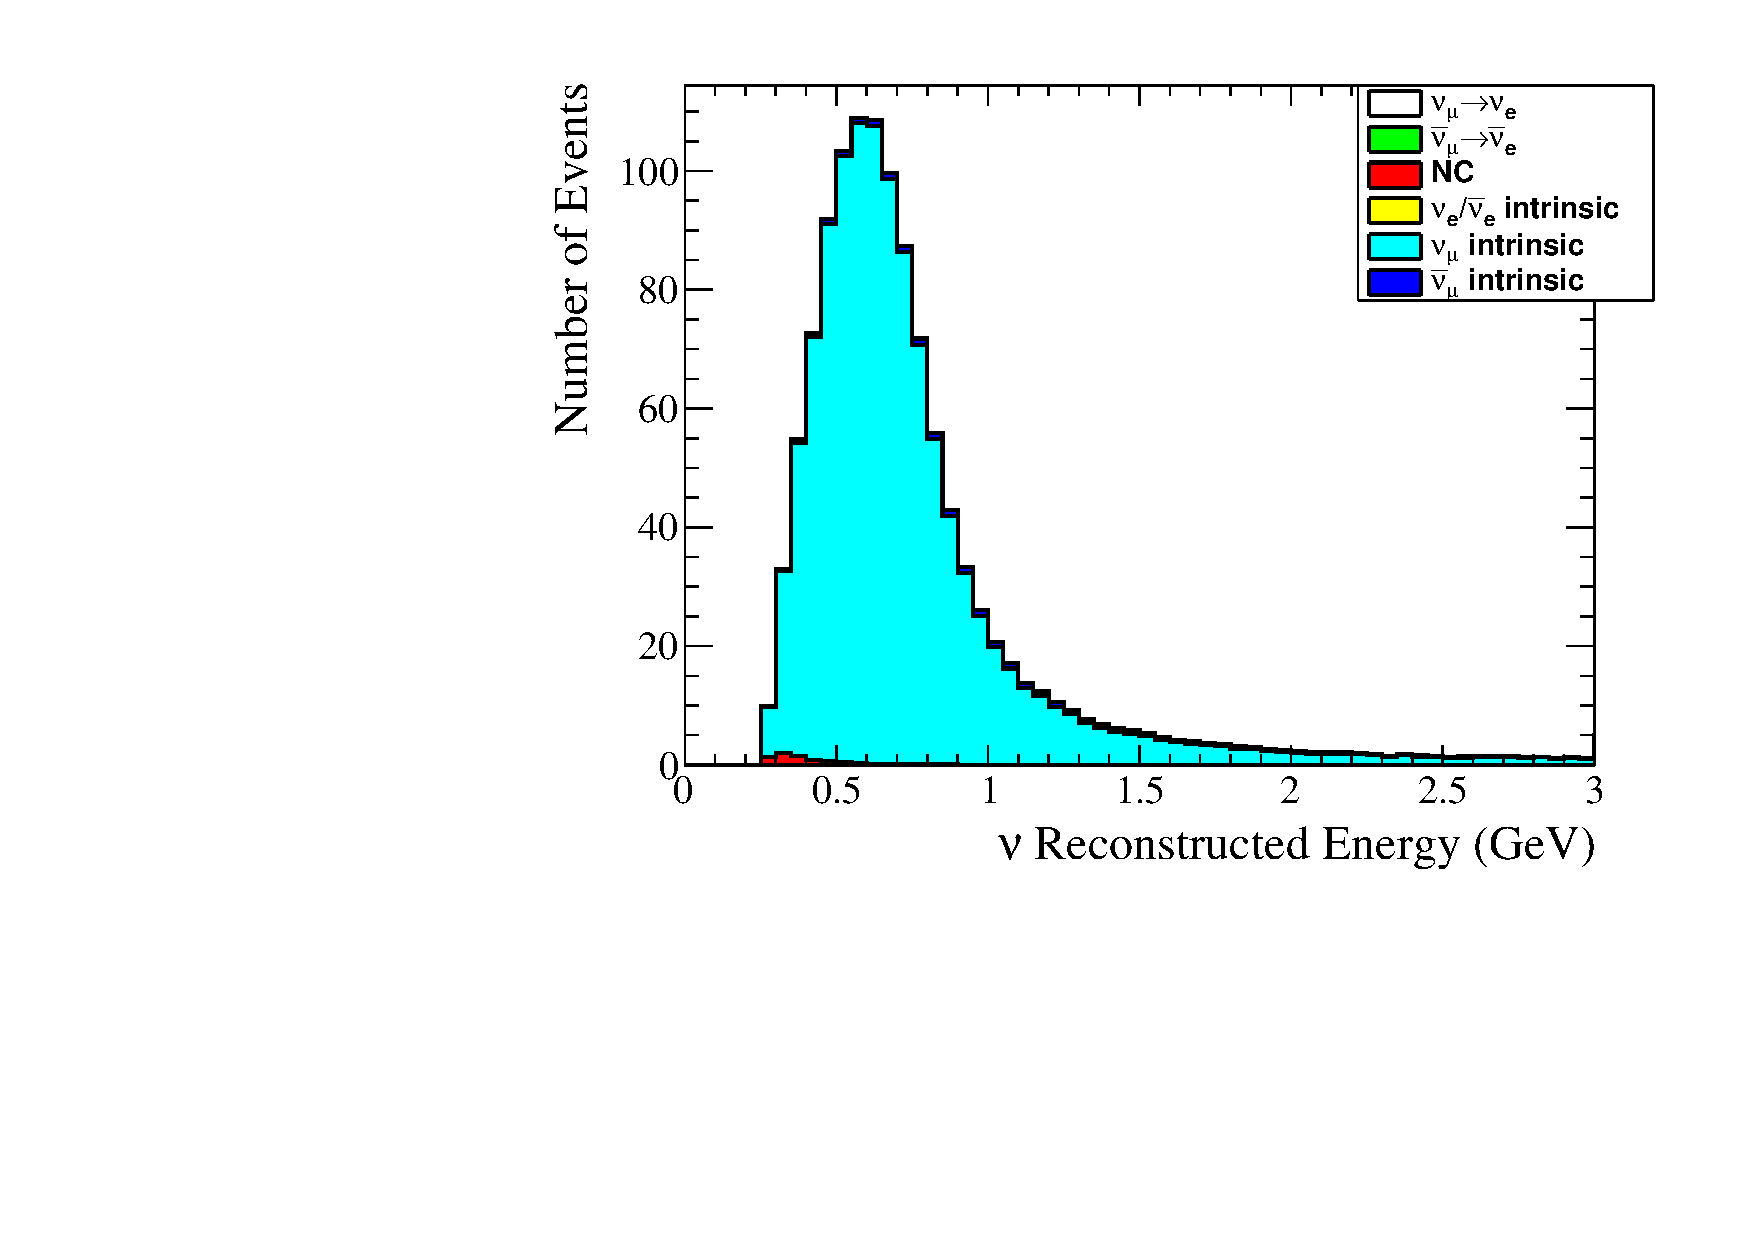
\includegraphics[width=0.9\textwidth]{spectra/spectrum_unosc_1Rmu}
		\caption{Muon-like, neutrino mode}
	\end{subfigure}
	\begin{subfigure}[b]{0.49\textwidth}
		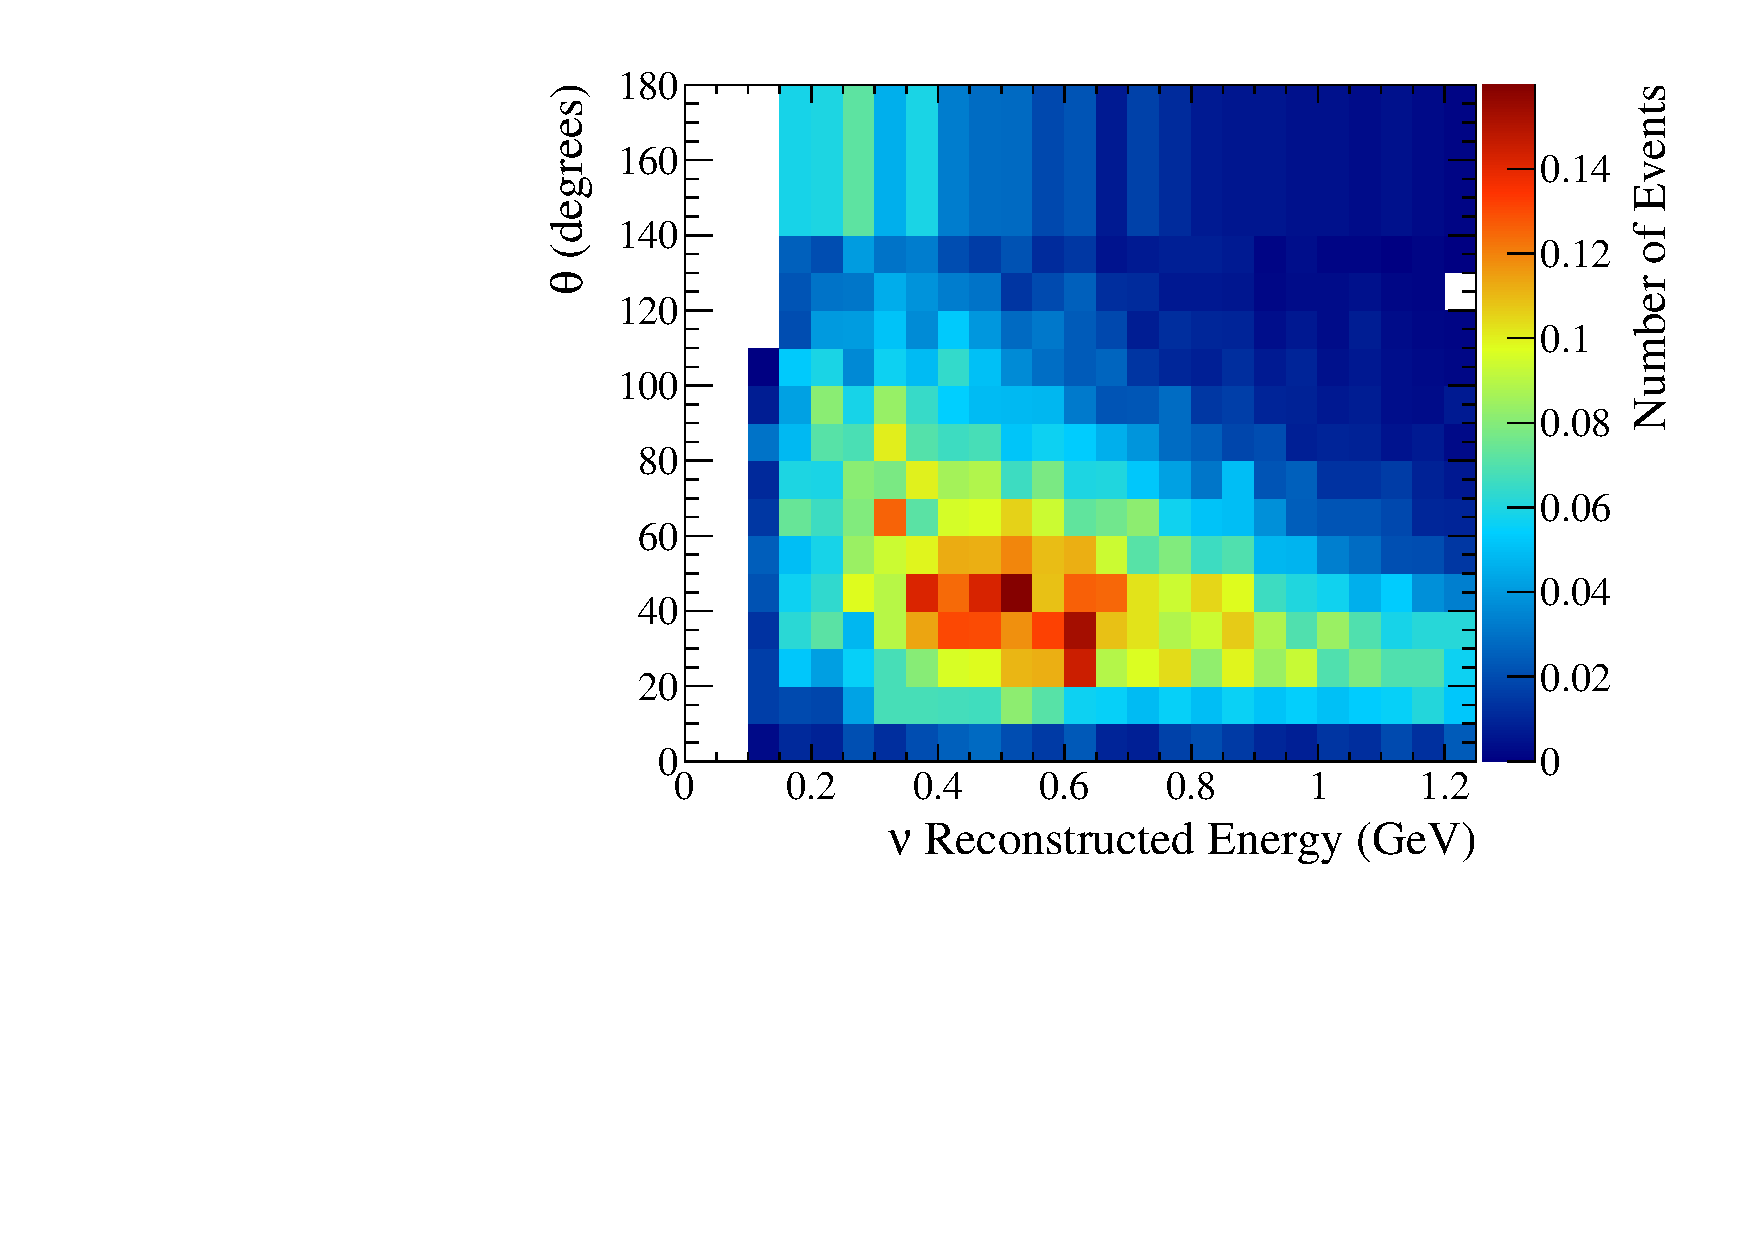
\includegraphics[width=0.9\textwidth]{spectra/spectrum_unosc_1Re}
		\caption{Electron-like, neutrino mode}
	\end{subfigure}
	\begin{subfigure}[b]{0.49\textwidth}
		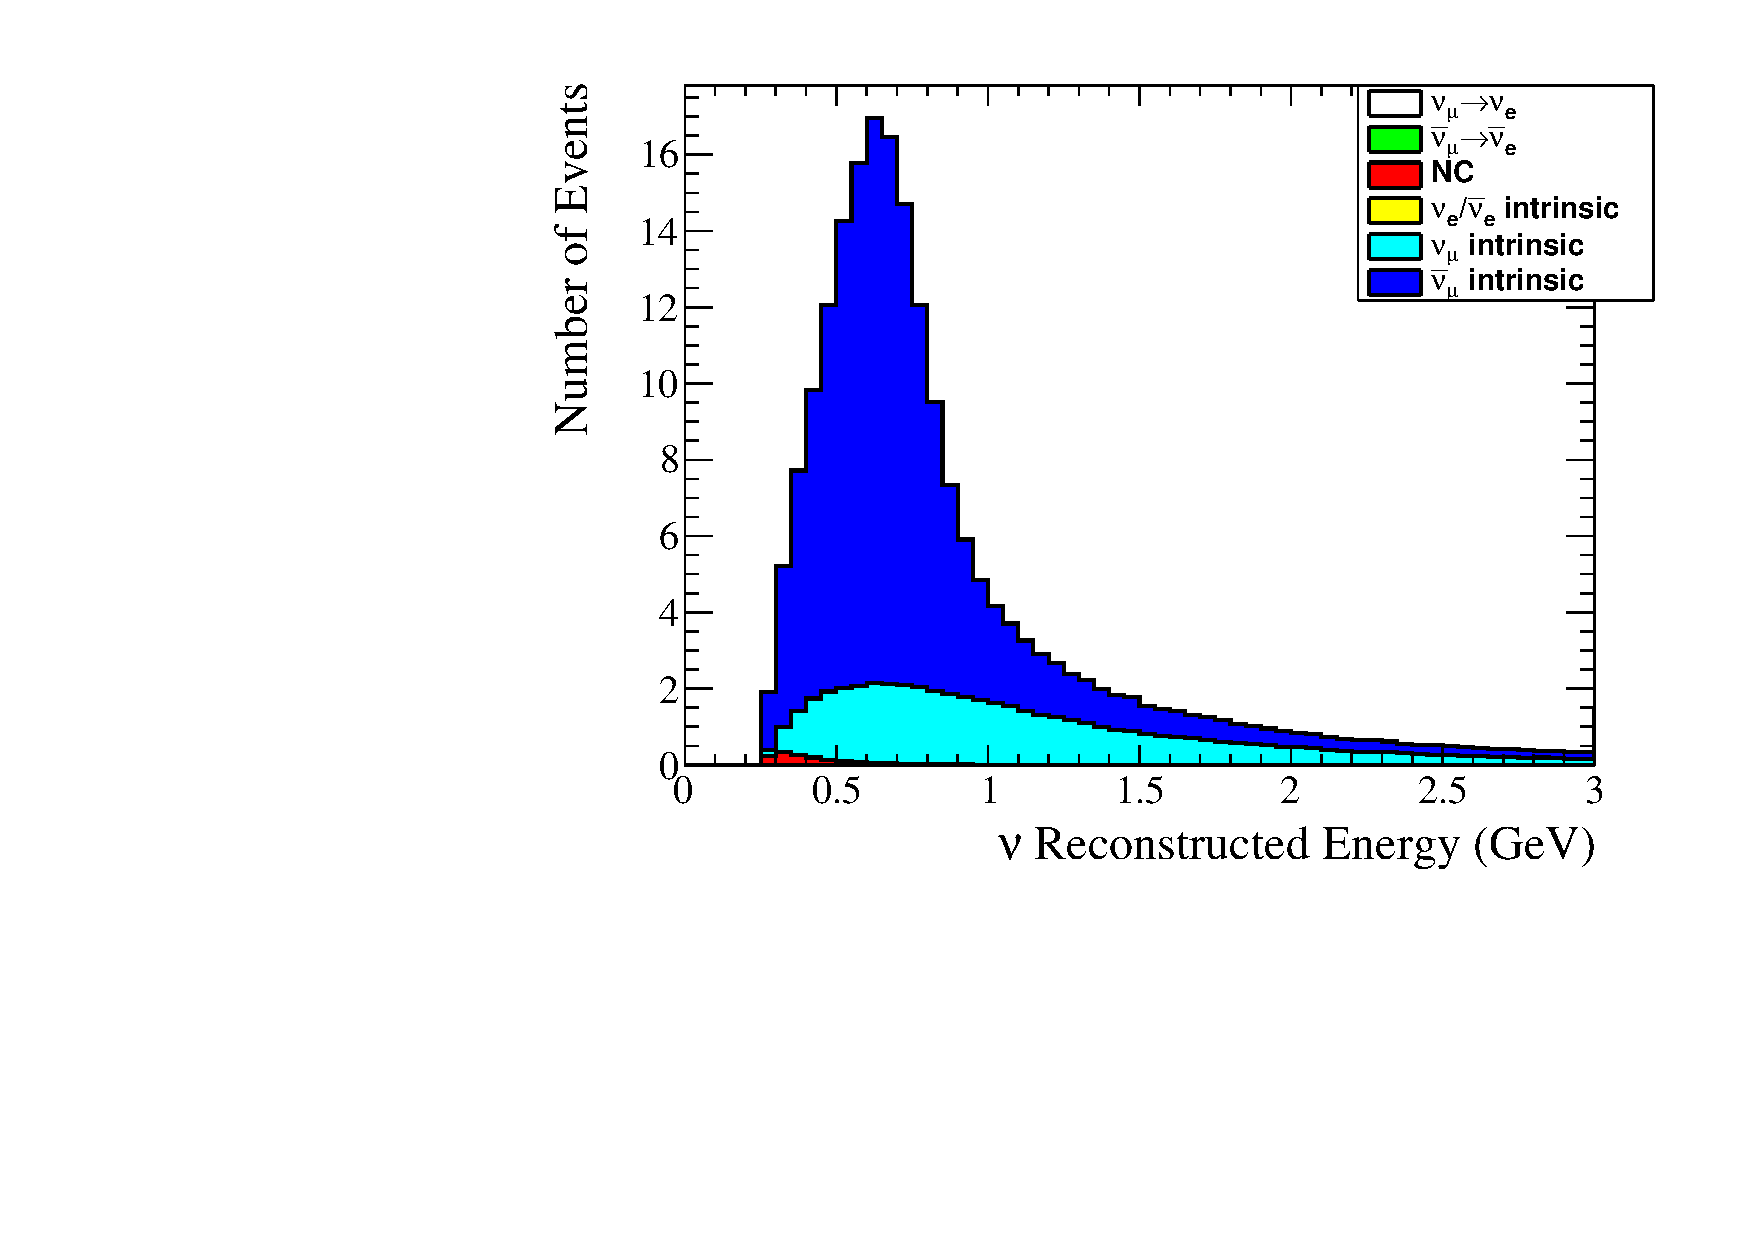
\includegraphics[width=0.9\textwidth]{spectra/spectrum_unosc_RHC1Rmu}
		\caption{Muon-like, antineutrino mode}
	\end{subfigure}
	\begin{subfigure}[b]{0.49\textwidth}
		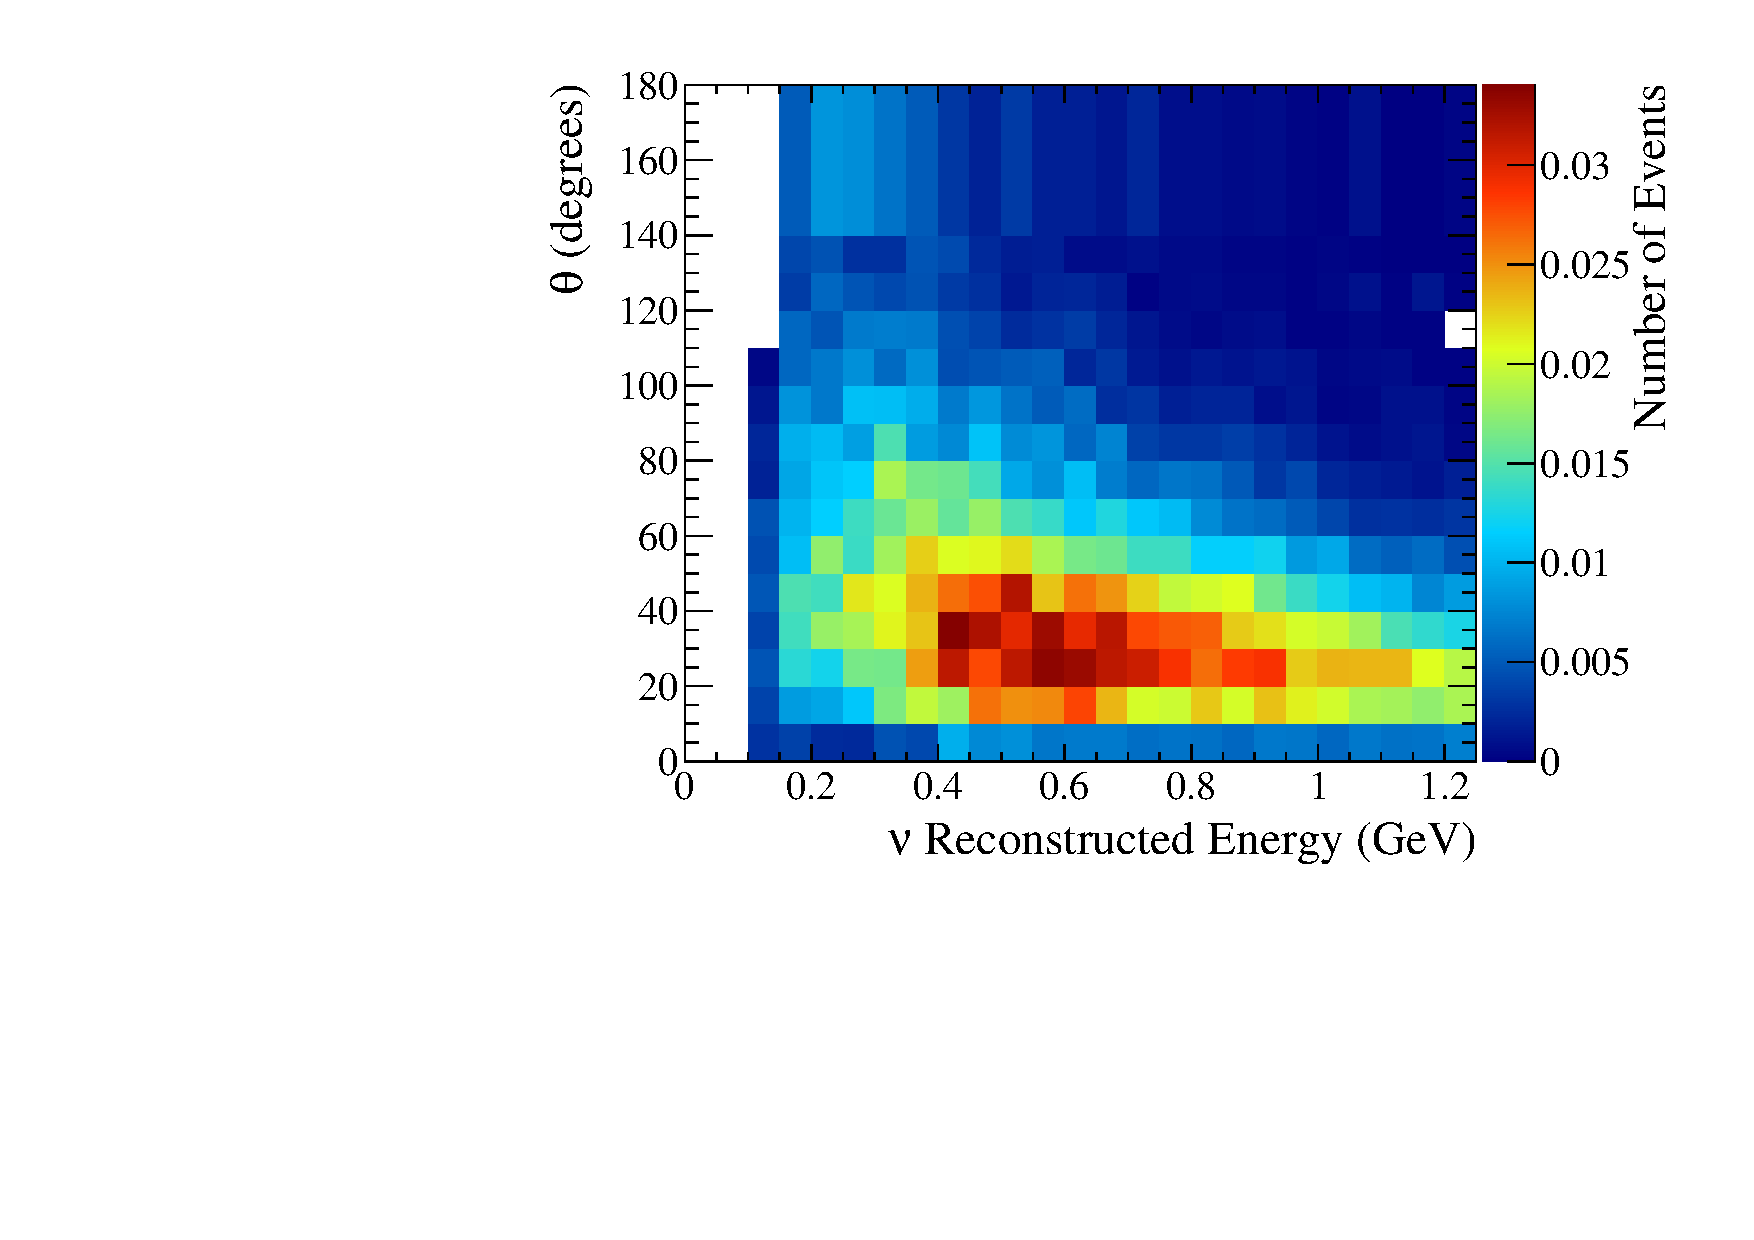
\includegraphics[width=0.9\textwidth]{spectra/spectrum_unosc_RHC1Re}
		\caption{Electron-like antineutrino mode}
	\end{subfigure}
	\begin{subfigure}[b]{0.49\textwidth}
		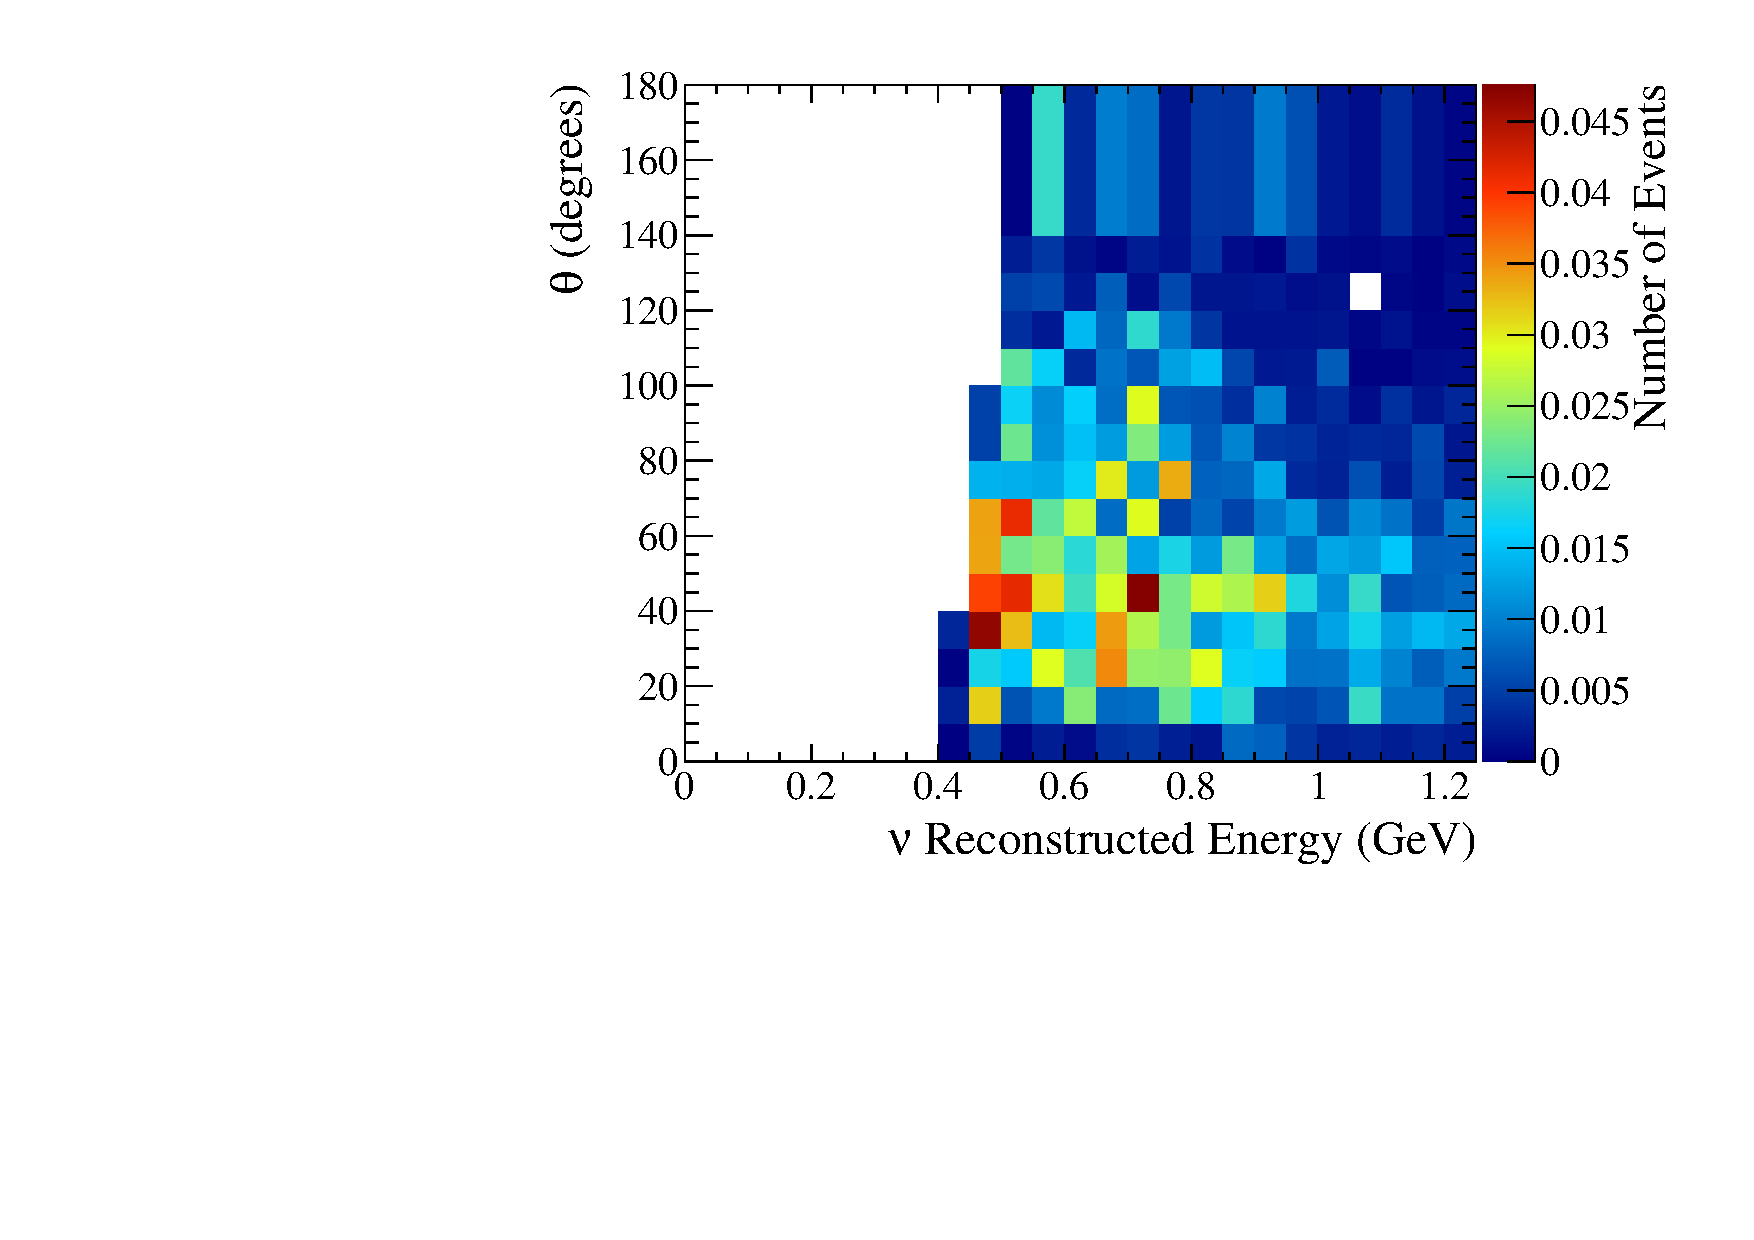
\includegraphics[width=0.9\textwidth]{spectra/spectrum_unosc_MultiRe}
		\caption{\nueCConepi-like, neutrino mode}
	\end{subfigure}
	\caption {
		Predicted unoscillated spectra. $\mu$-like distributions are a function of the reconstructed neutrino energy, while the $e$-like, including \nueCConepi, distributions are functions of both the reconstructed neutrino energy and the reconstructed angle between the outgoing lepton and the neutrino direction. The distributions correspond to the statistics collected in the full \RunPeriod data set. The spectra are generated with the systematic parameters described in \cref{sec:systematics}.
	}
	\label{fig:unosc_spectra_all}
\end{figure*}
\clearpage
\begin{figure*}[htb]
	\center
	\begin{subfigure}[b]{0.49\textwidth}
		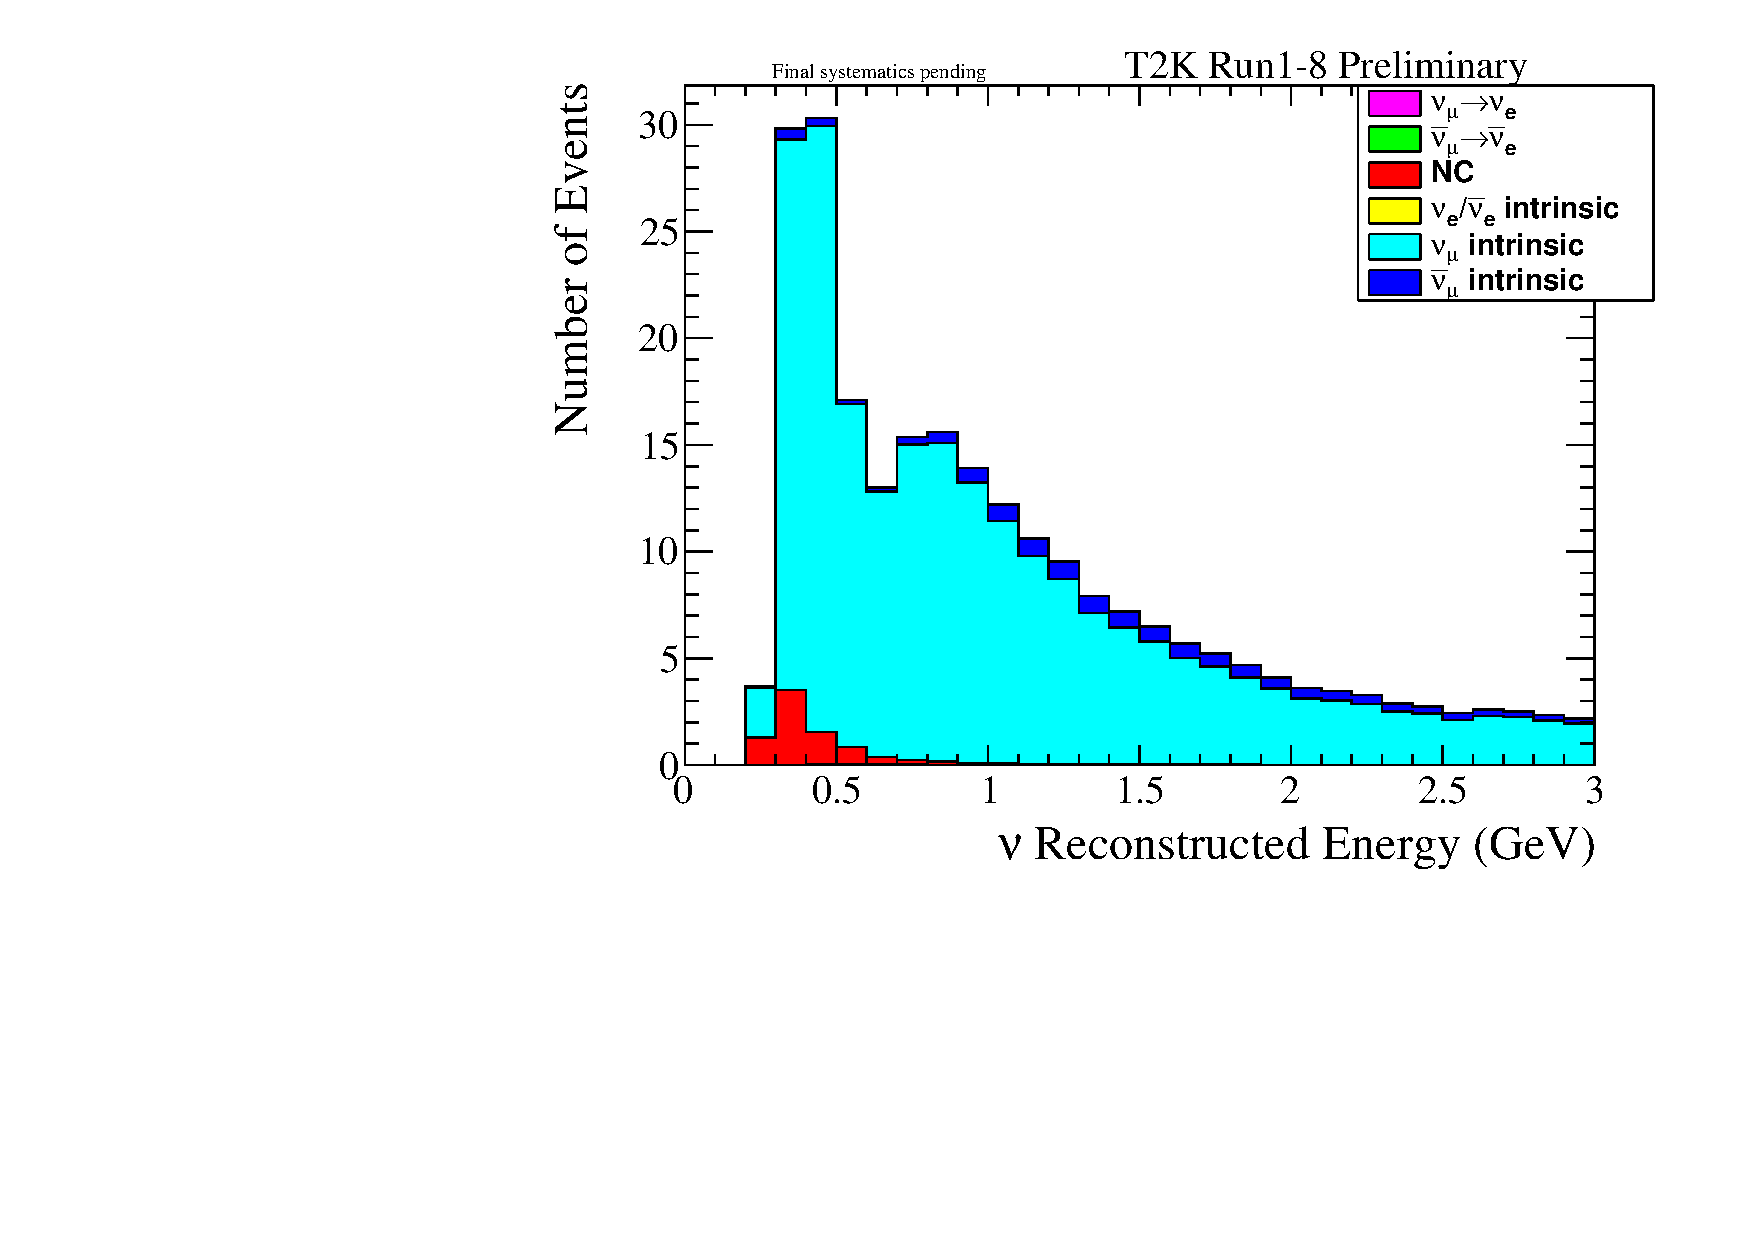
\includegraphics[width=0.9\textwidth]{spectra/spectrum_osc_asimova_1Rmu}
		\caption{Muon-like, neutrino mode}
	\end{subfigure}
	\begin{subfigure}[b]{0.49\textwidth}
		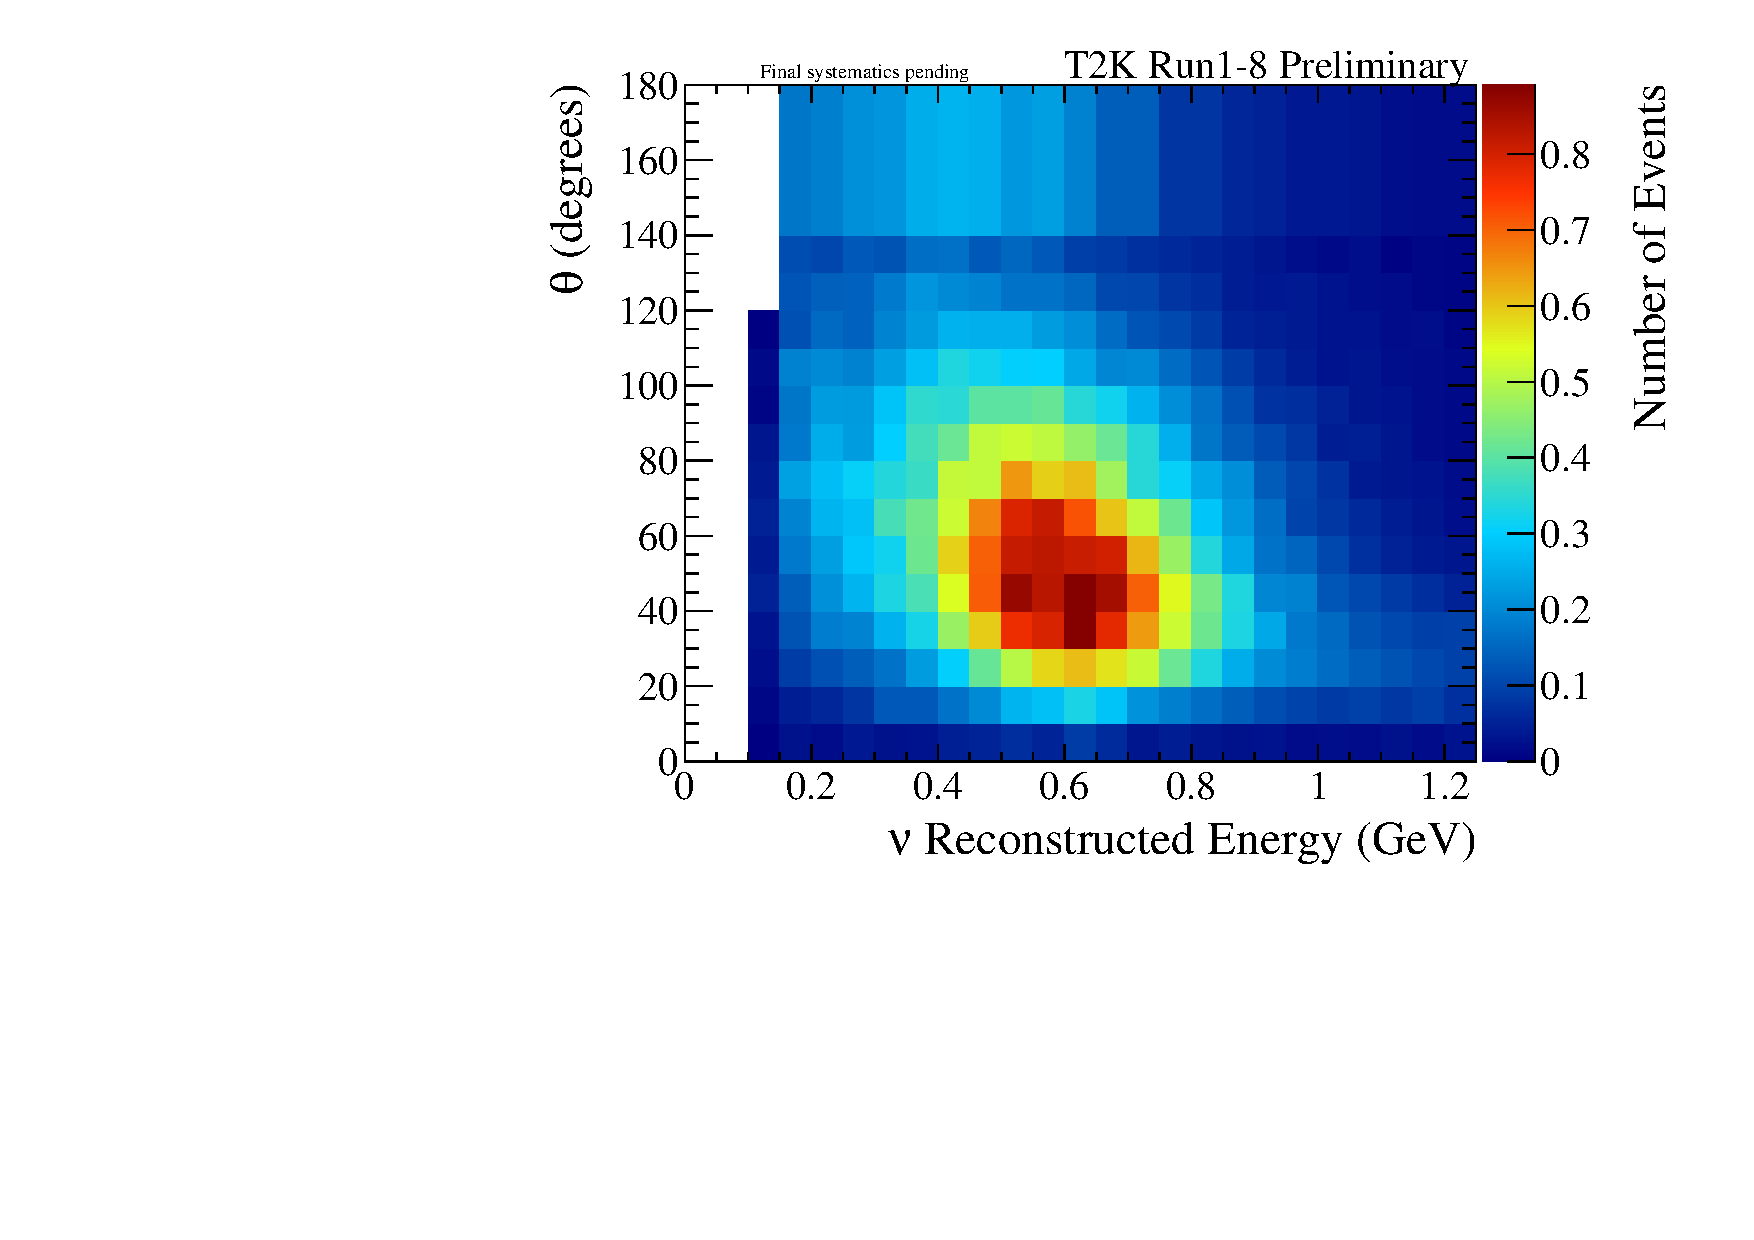
\includegraphics[width=0.9\textwidth]{spectra/spectrum_osc_asimova_1Re}
		\caption{Electron-like, neutrino mode}
	\end{subfigure}
	\begin{subfigure}[b]{0.49\textwidth}
		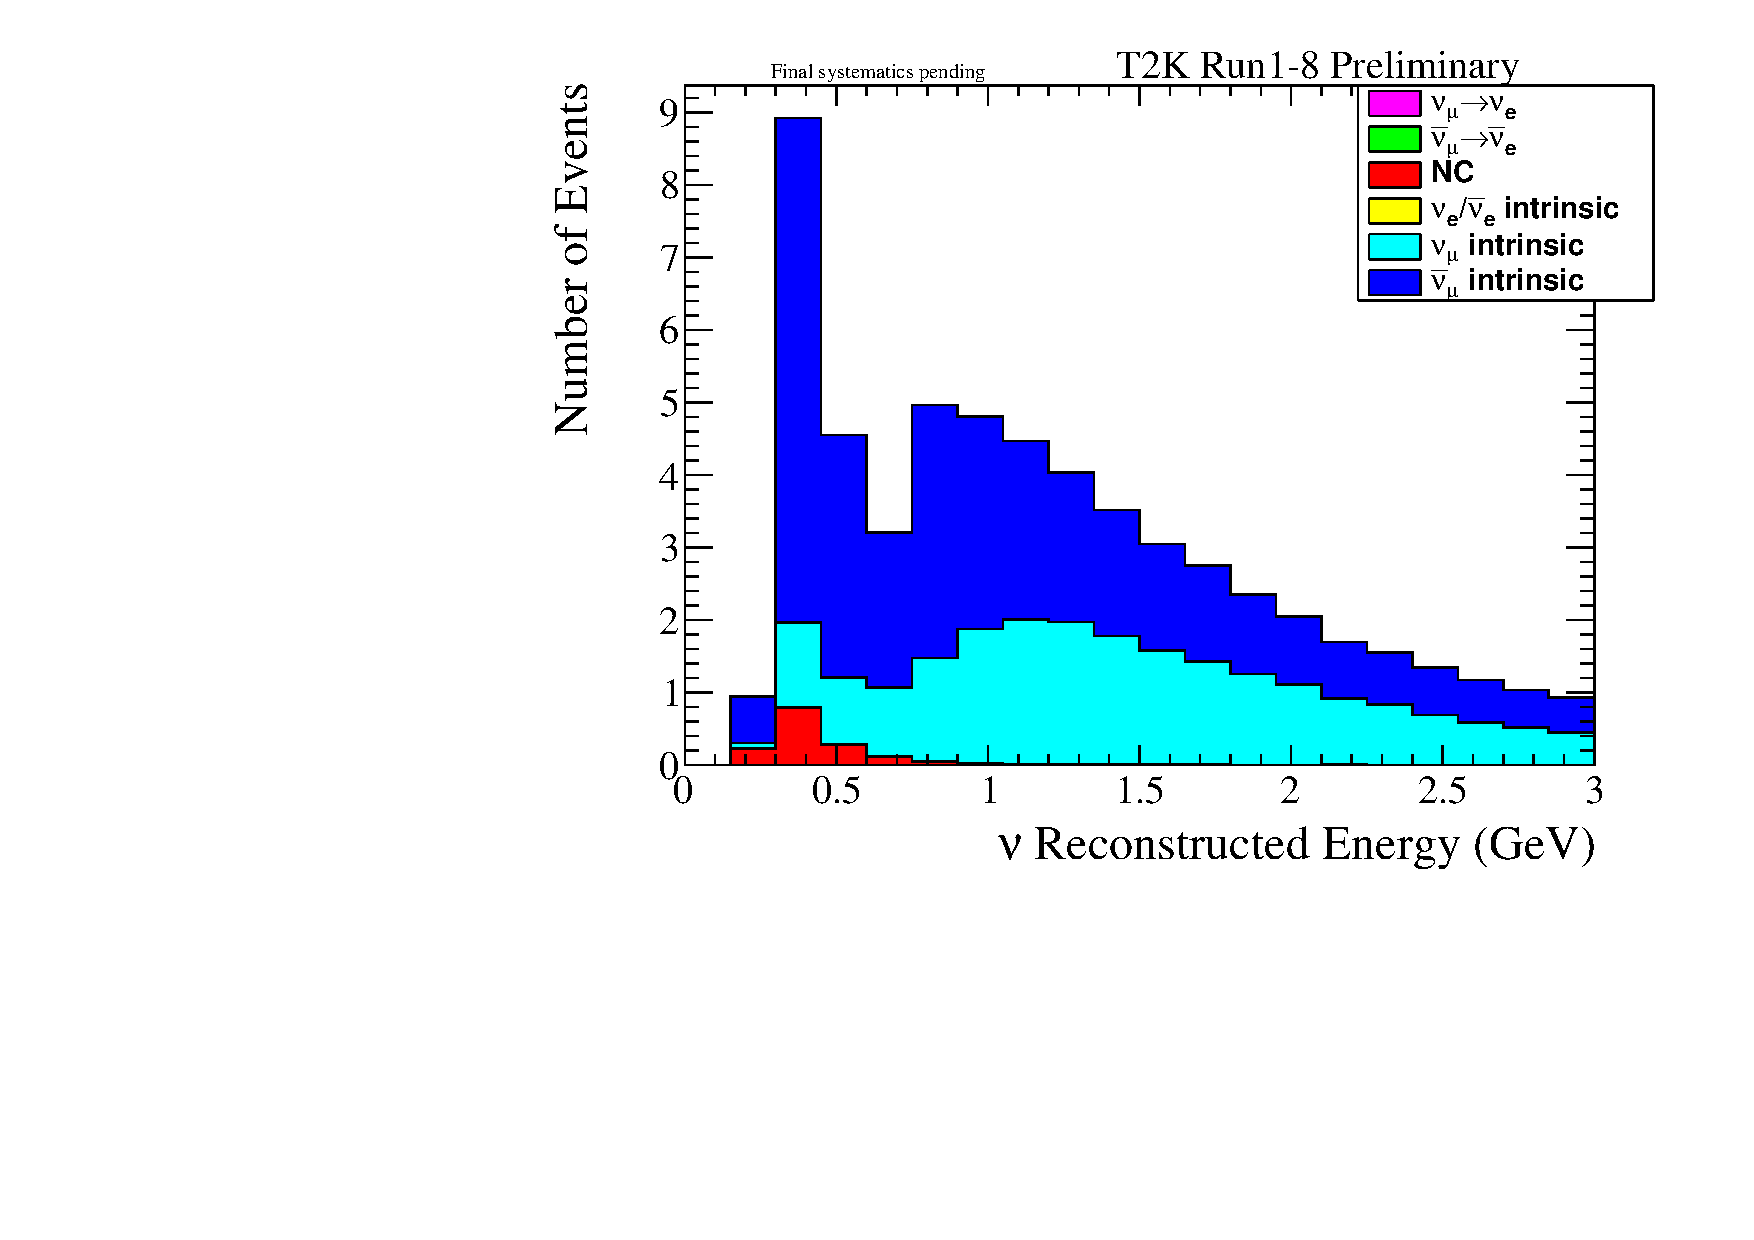
\includegraphics[width=0.9\textwidth]{spectra/spectrum_osc_asimova_RHC1Rmu}
		\caption{Muon-like, antineutrino mode}
	\end{subfigure}
	\begin{subfigure}[b]{0.49\textwidth}
		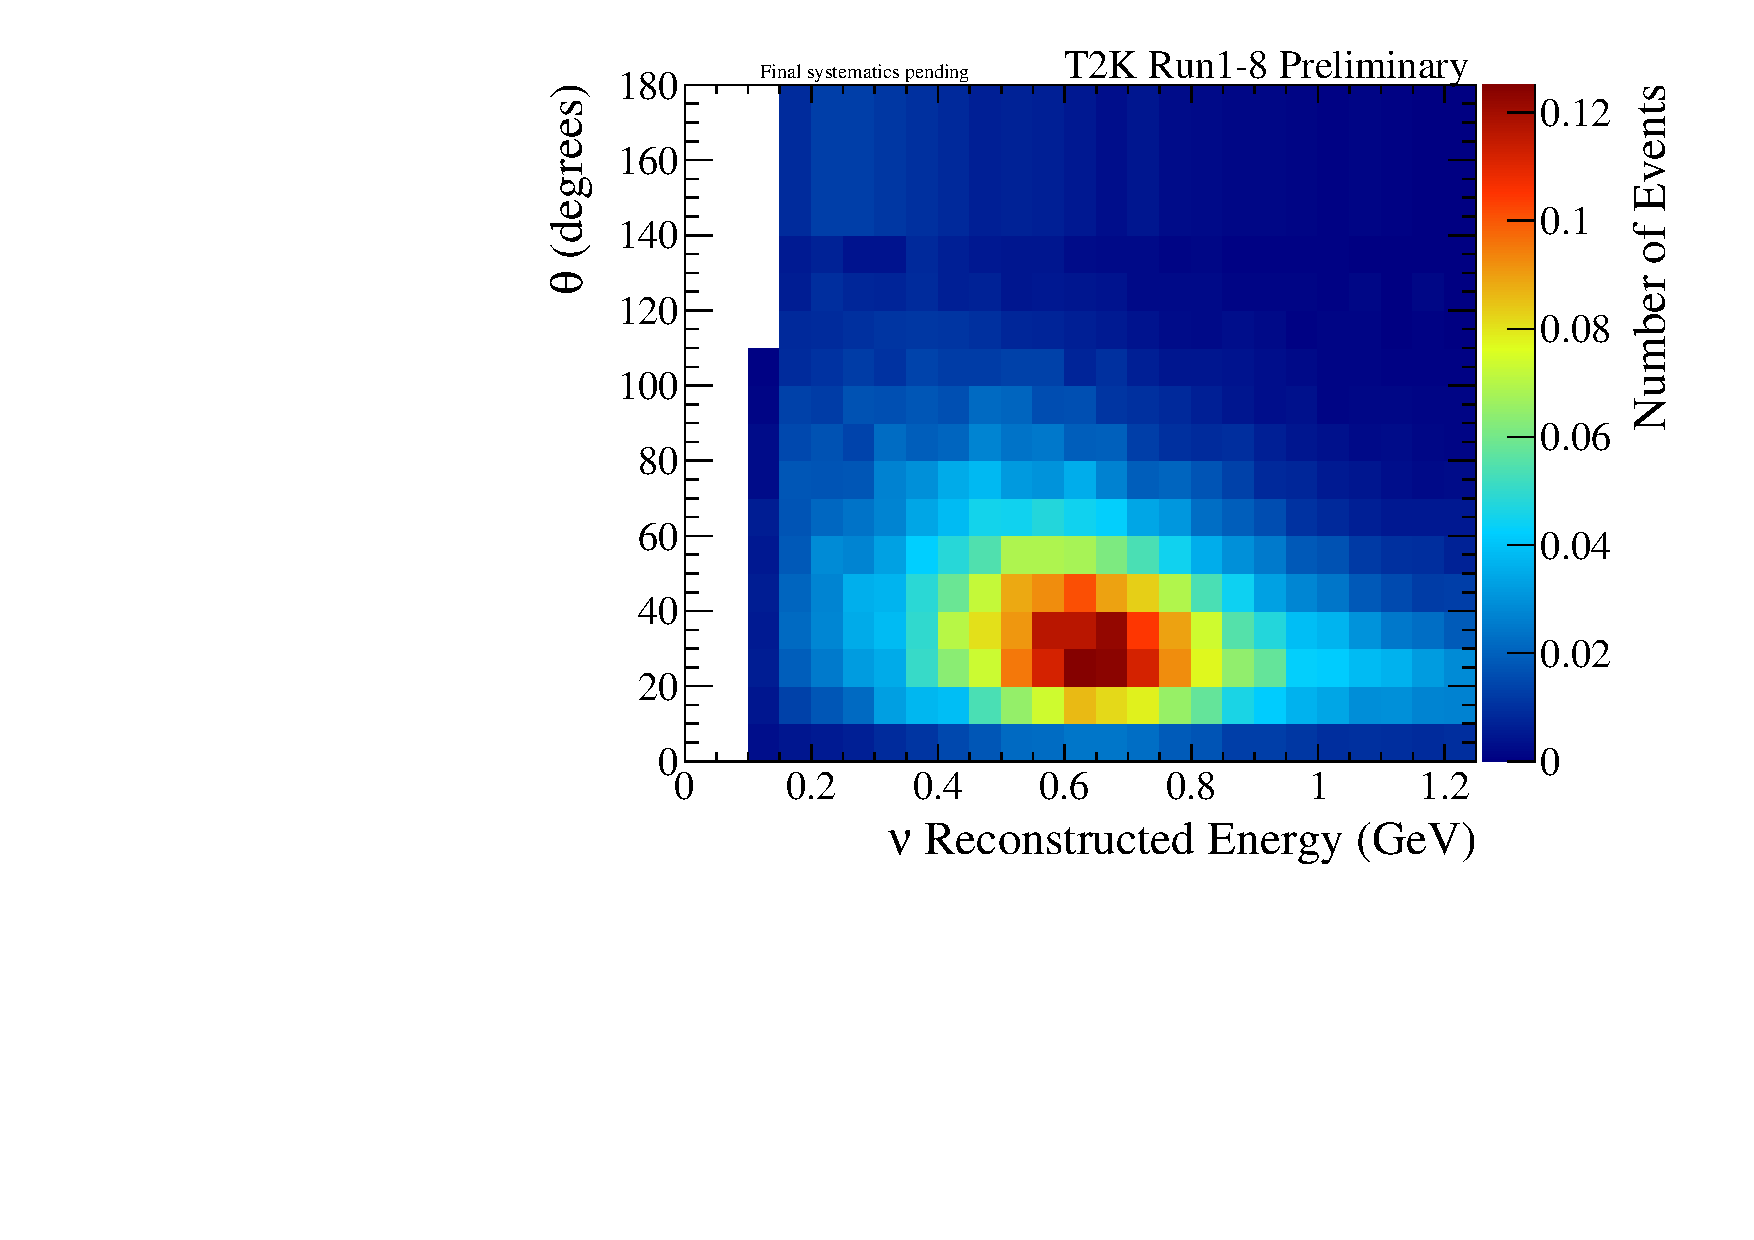
\includegraphics[width=0.9\textwidth]{spectra/spectrum_osc_asimova_RHC1Re}
		\caption{Electron-like antineutrino mode}
	\end{subfigure}
	\begin{subfigure}[b]{0.49\textwidth}
		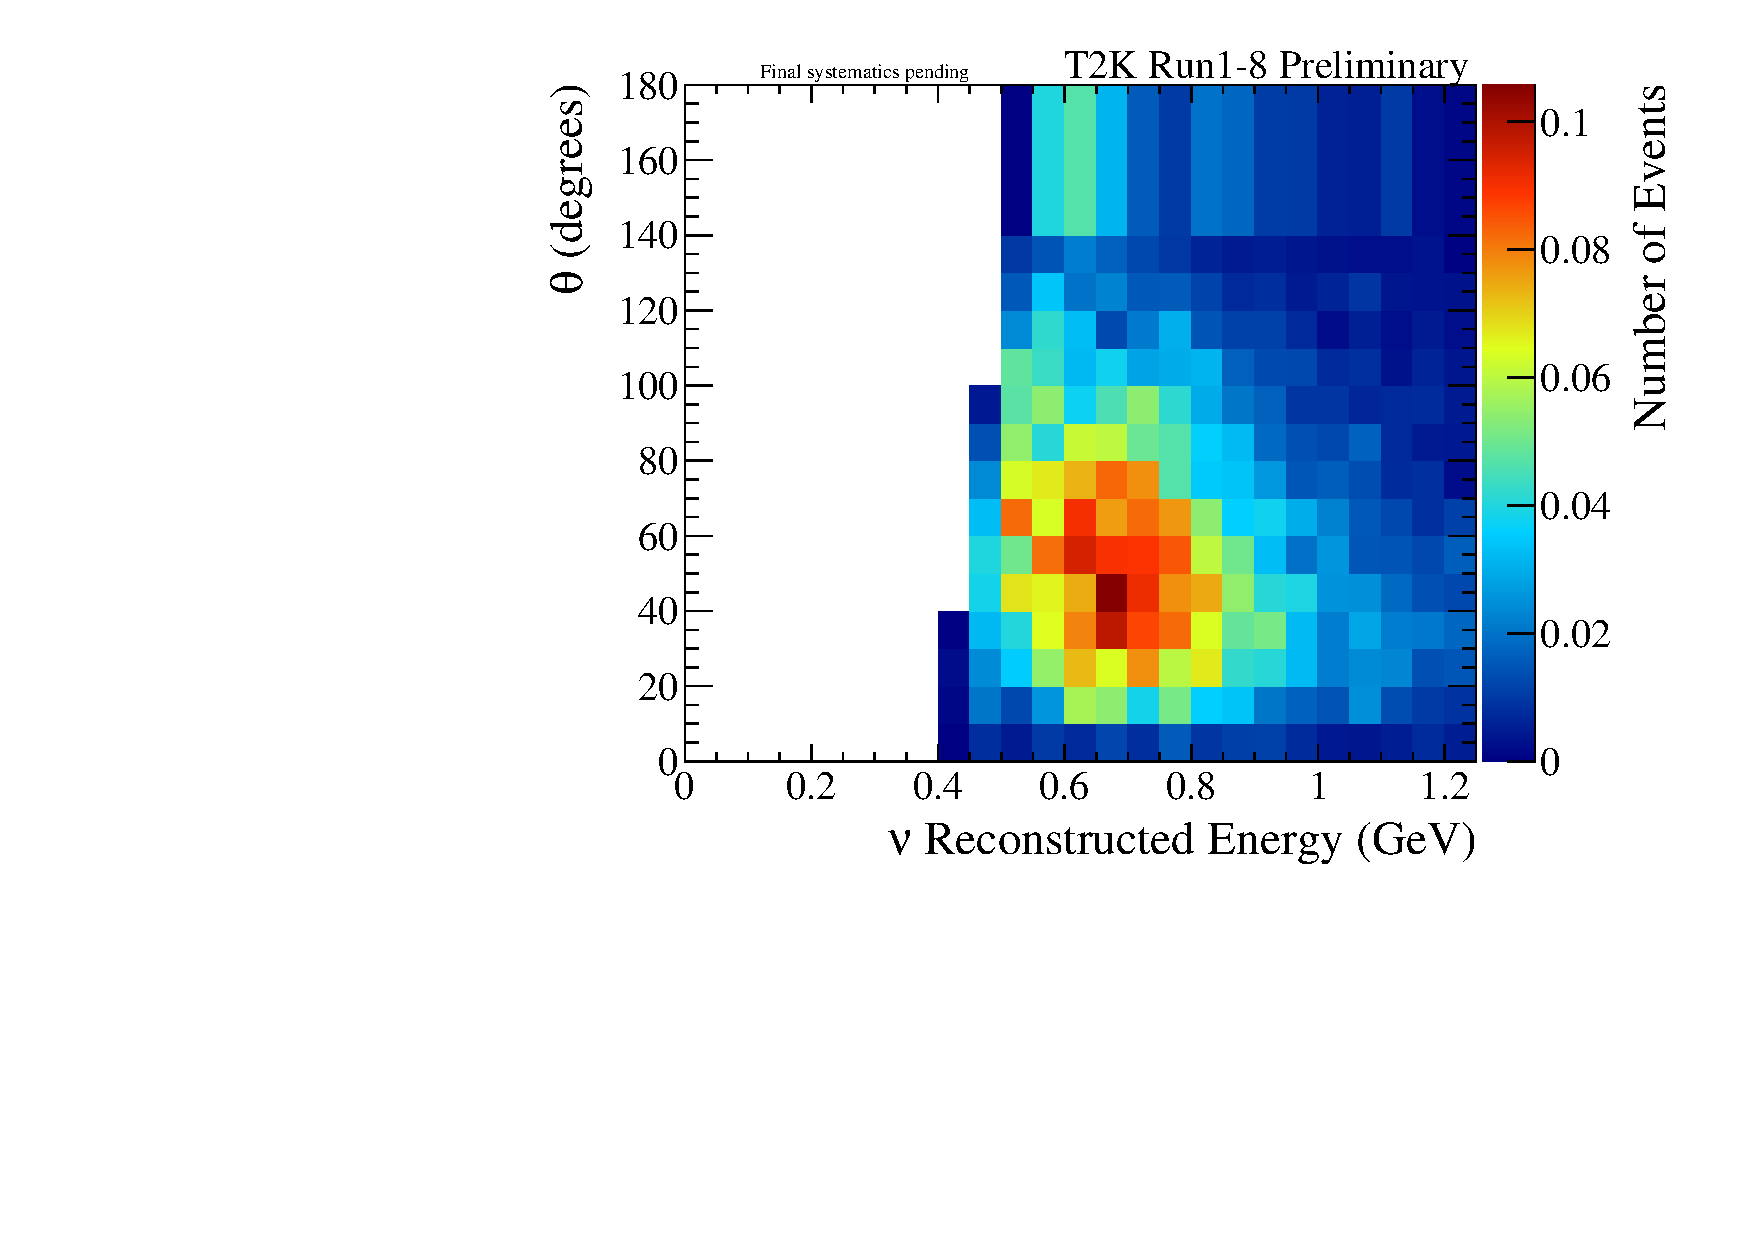
\includegraphics[width=0.9\textwidth]{spectra/spectrum_osc_asimova_MultiRe}
		\caption{\nueCConepi-like, neutrino mode}
	\end{subfigure}
	\caption {
		Predicted Asimov A spectra. $\mu$-like distributions are a function of the reconstructed neutrino energy, while the $e$-like, including \nueCConepi, distributions are functions of both the reconstructed neutrino energy and the reconstructed angle between the outgoing lepton and the neutrino direction. The distributions correspond to the statistics collected in the full \RunPeriod data set. The spectra are generated with the systematic parameters described in \cref{sec:systematics} and the oscillation parameters corresponding to the Asimov data set A shown in \cref{tab:asimov_definition1}.
	}
	\label{fig:asimova_spectra_all}
\end{figure*}
\clearpage